% !TEX root = ../../../../thesis.tex

\section{Natural Computing with \P}\label{sec:natural_computing_physarum}

	Starting with the year 2000 a series of break-through experiments caused the unassuming organisms that are slime molds to become the focus of intense research efforts. In particular, it was demonstrated that in its plasmodium stage, \P is capable of reacting to environmental conditions in a manner that is reminiscent of optimization processes. Examples include the maximization of food uptake given a small set of food sources, or the minimization of exposure to light known to be harmful to the organism. It is striking that there is no central control coordinating these nontrivial processes. Since \P lacks any sort of brain or nervous system, it has been speculated that the observed capabilities are emergent as a result of local interactions. Given its abilities, \P can be seen as a highly distributed system with properties suitable for distributed natural computing.

	In order to explain the behavior of \P and to harness its in-built optimization capabilities, several different approaches were put forward. The most successful amongst those either focus on modeling certain key observations that were discovered experimentally or manipulate the organism \textit{in vivo} in such a way that its behavior can be interpreted as computation. In the next section we survey some of the most influential experiments which paved the way for natural computing with \P.

	\subsection{Key Experiments and Observations}

		\subsubsection{Emergence of Synchronization in \P }\label{sec:oscillator_experiment}
		
			In the last decade of the 20th century the rhythmic contractions exhibited by the plasmodium of \P were the subject of a series of experiments aimed at shedding light onto the basic mechanisms governing \P~\cite{MIYAKE1996341,NAKAGAKI1996261,TAKAHASHI1997105}. Soon it was established that mechanochemical reactions among intracellular chemicals such as ATP and calcium generate periodic cycles of contraction and relaxation of actomyosin fibers, explaining the observed oscillations in the thickness of the plasmodium. Periodic changes in thickness induce pressure differences between different parts of the slime mold which cause protoplasmic fluid to be streaming to and fro, exhibiting periodic reversals of direction. Given the experimental findings it seemed natural to view the plasmodium of \P as an ensemble of coupled non-linear oscillators. Using this Ansatz, mutual entrainment of intracellular oscillators may give rise to self-organization and the information processing capabilities of \P. 

			In this context, a key experiment was presented in 2000 which uses the plasmodium of \P to realize a living system of coupled oscillators~\cite{PhysRevLett.85.2026}. To this end a micro-fabricated structure was prepared, consisting of two identical circular reservoirs, connected by a channel of a predetermined width and length. In the experiment, the two reservoirs and the channel are populated with plasmodium. The reservoirs act like two distinct \P oscillators while the channel ensures a controllable coupling between the two. Here the width of the channel represents the coupling strength while the length of the channel corresponds to the time delay in the coupling. The setup depicted in \Fref{fig:oscillator_experiment_setup} realizes a system of two delay-coupled oscillators whose thickness oscillations were studied as a function of the channel dimensions.

			\begin{figure}[htb]
				\centering
				\subfloat[Oscillator experiment - Plasmodium][]{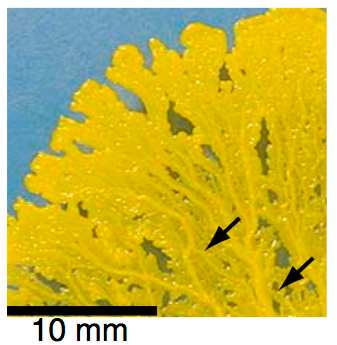
\includegraphics[width=\twoimageswide,keepaspectratio]{oscillator/plasmodium.png}}
				\subfloat[Oscillator experiment - Microfabricated structure loaded with plasmodium][]{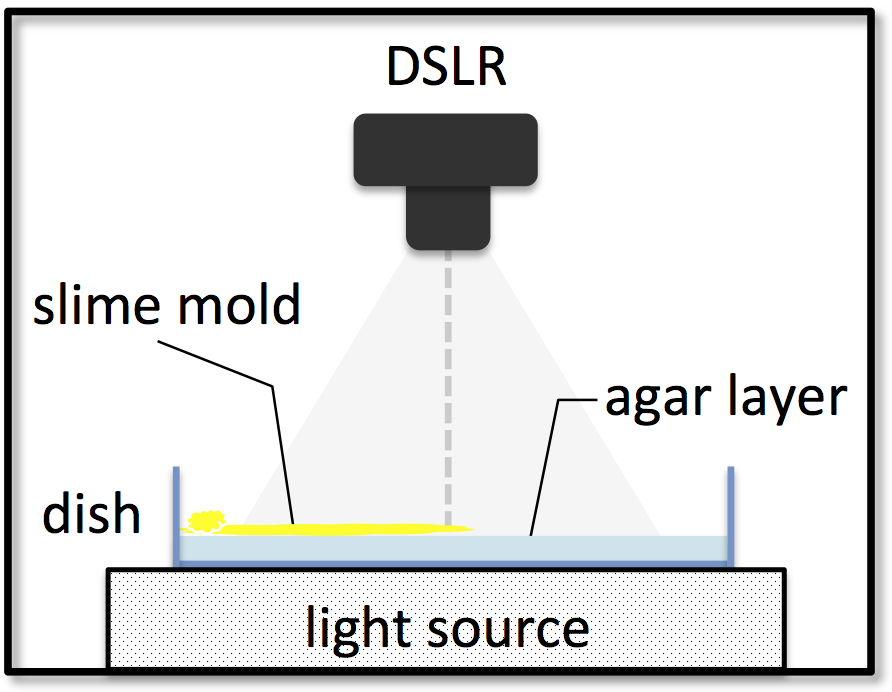
\includegraphics[width=\twoimageswide,keepaspectratio]{oscillator/setup.png}}
	
				\caption[Oscillator experiment - Setup]{(a) Detail of the growing front of \P. Arrows indicate the presence of thick veins. (b) Top: A micro-fabricated structure designed to confine \P. The diameter of the reservoirs was chosen such that they can be regarded as distinct oscillators. Bottom: The dumbbell shaped structure loaded with \P. Reprinted from~\cite{PhysRevLett.85.2026}.}
				\label{fig:oscillator_experiment_setup}
			\end{figure}

			\Fref{fig:oscillator_experiment_thickness} shows rich self-synchronizing oscillation patterns exhibiting both in-phase and anti-phase entrainment consistent with theoretical expectations. The experiment shows that the geometry of the channel plays a key role in the generation of thickness oscillations driving peristaltic pumping of protoplasm.

			\begin{figure}
				\centering
				\subfloat[Oscillator experiment - Thickness oscillations visualized][]{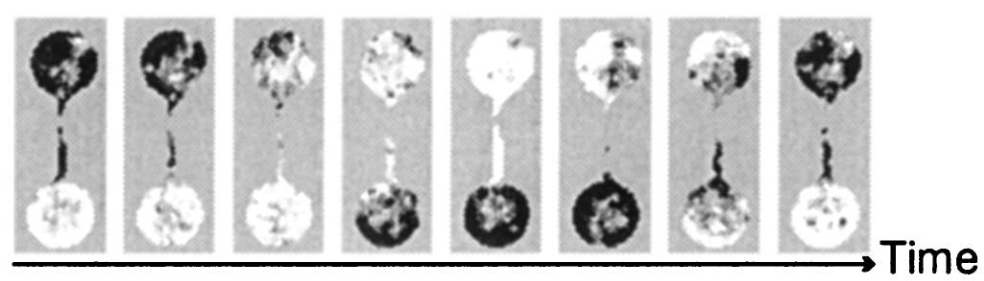
\includegraphics[width=\oneimagewide,keepaspectratio]{oscillator/thickness_oscillations.png}}
				\newline
				\subfloat[Oscillator experiment - Thickness oscillations over time][]{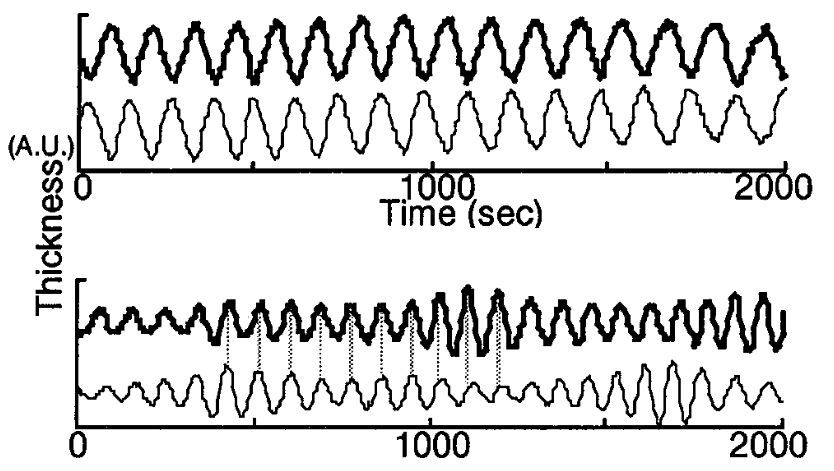
\includegraphics[width=\oneimagewide,keepaspectratio]{oscillator/thickness_oscillations_graph.png}}
	
				\caption[Oscillator experiment - Thickness oscillations]{(a) Visualization of thickness anti-phase oscillations propagating between the two oscillators by means of the transmitted light intensity through the plasmodium. Darker/brighter areas indicate an increase/decrease in thickness. The time interval between consecutive images is \SI{16}{\second}. (b) Time development of thickness oscillations. The thick respectively thin lines represent the thickness of individual oscillators obtained by averaging the transmitted light intensity for each oscillator.
				Top: Anti-phase oscillations were observed for $W=\SI{0.4}{\milli\metre}$ and $L=\SI{4}{\milli\metre}$. Bottom: In-phase oscillations were observed for $W=\SI{0.5}{\milli\metre}$ and $L=\SI{010}{\milli\metre}$. Adapted and reprinted from~\cite{PhysRevLett.85.2026}.}
				\label{fig:oscillator_experiment_thickness}
			\end{figure}{}

			\FloatBarrier

		\subsubsection{Shortest Path in a Maze}

			Introduced in the year 2000, in the so-called ``maze experiment'', the plasmodium of \P is introduced to a maze, see \Fref{fig:maze:initial}~\cite{nakagaki2000intelligence}. After the plasmodium has spread evenly across the entire maze, two food sources are introduced at two specific points in the maze, see \Fref{fig:maze:intermediate}. The organism reacts to the food source by slowly retracting from areas of the maze that do not coincide with any path connecting them. This process continues for several hours until the plasmodium takes the shape of one single thick vein connecting the food sources. In repeated experiments, it was shown that after sufficient time this vein does not occupy any path, but selects the shortest path ($\alpha_1 + \beta_1$, see \Fref{fig:maze:initial}) in most of the cases. This demonstrates the organisms remarkable ability to iteratively improve the efficiency of fluid flow between the two food sources. By making veins progressively shorter and wider, the hydrodynamic resistance to protoplasmic flow is minimized which is beneficial in terms of nutrient transport\cite{kamiya1959motive}. 

			In terms of natural computing, one may interpret the maze as a graph with edge weights equal to the lengths of the associated maze segments and the food sources as two distinct nodes $N_1$ and $N_2$, see~\Fref{fig:maze:abstraction}. Thus the slime mold \Pp can be seen to demonstrate an \emph{in vivo} approximate solution to the $s-t$ shortest path problem with $s=N_1$ and $t=N_2$. 

			\begin{figure}
				\centering
				\subfloat[Maze experiment - Initial state][]{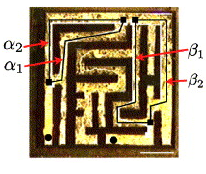
\includegraphics[width=\twoimageswide,keepaspectratio]{maze/maze_experiment_1.png}\label{fig:maze:initial}}
				\subfloat[Maze experiment - Intermediate state][]{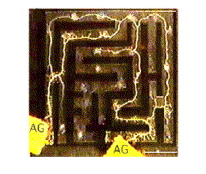
\includegraphics[width=\twoimageswide,keepaspectratio]{maze/maze_experiment_2.png}\label{fig:maze:intermediate}}
				\newline
				\subfloat[Maze experiment - Final state][]{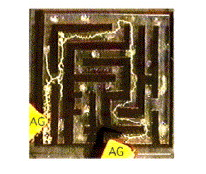
\includegraphics[width=\twoimageswide,keepaspectratio]{maze/maze_experiment_3.png}\label{fig:maze:final}}
				\subfloat[Maze experiment - Graph abstraction][]{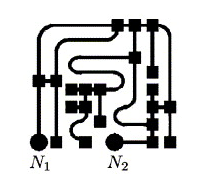
\includegraphics[width=\twoimageswide,keepaspectratio]{maze/maze_experiment_4.png}\label{fig:maze:abstraction}}
				
				\caption[Classic maze experiment with \P]{ (a) The plasmodium of 
				\P is evenly spread across a maze. Filled black circles denote two specific points in the maze. Arrows indicate segments of possible paths between them. (b) Two food sources, labeled \textbf{\texttt{AG}}, are introduced at the specific points. After a while the plasmodium retreats from areas of the maze that do not intersect with a path connecting the food sources. (c) The plasmodium settles on the shortest path between the two food sources. (d) The maze can be interpreted as an abstract graph with two distinct nodes $N_1$ and $N_2$ corresponding to the food sources. The scale bars denote \SI{1}{\centi\metre}. Reprinted from~\cite{Tero2007553}.}
				\label{fig:maze}
			\end{figure}

			\FloatBarrier

		\subsubsection{Efficient networks maximizing food uptake given multiple food sources}

			In 2004 the plasmodium of \P was presented with multiple food sources arranged in various regular patters including equilateral triangles and small grids~\cite{Nakagaki20041,nakagaki2004obtaining}. Independent of the chosen pattern, the organism reacted by changing its shape from a sheetlike plasmodium to a distinct network featuring thick veins. This network was found to balance two competing yet desirable features. Namely, small total length of the tubular network and high tolerance against accidental loss of connectivity. The first feature implies that the biomass required for maintaining veins be small. As a result the bulk of the biomass may concentrate on the food sources themselves in order to improve food uptake. The second feature makes sure that the organism is not disconnected after severing a small number of veins. This allows the organism to keep exploiting obtained food sources and information as a unit. Such behavior is crucial for instance, if a remote part of the vein networks senses an unclaimed food source. Then this information may be processed by the entire organism leading to a potential redistribution of biomass, enabling further improvement of food uptake. If the part which discovers the new food source is disconnected from the main body, the latter cannot react to benefit from the discovery.

			Experimentally it was found that the networks formed by \P resemble minimum Steiner trees with additional cycles contributing a degree of fault tolerance, see \Fref{fig:steiner_tree_experiment}. The authors allow however, that the approximate Steiner points are likely to be a mere byproduct of searching for short connections between food sources. The inherent capability of forming functional networks was demonstrated impressively in another experiment where \P was set up to approximate the railway area of Tokyo and the greater Kanto area~\cite{tero2010rules}.

			\begin{figure}
				\centering
				\subfloat[Network formation experiment - Approximate MST][]{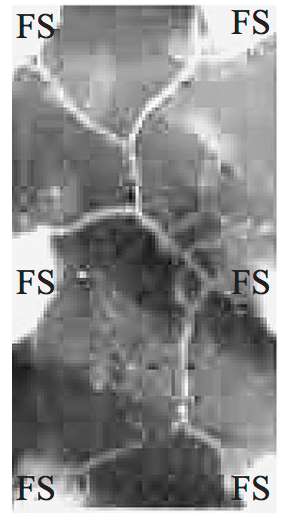
\includegraphics[height=0.3\textheight,keepaspectratio]{mst/mst_a.png}}
				\subfloat[Network formation experiment - Approximate MST with additional cycles][]{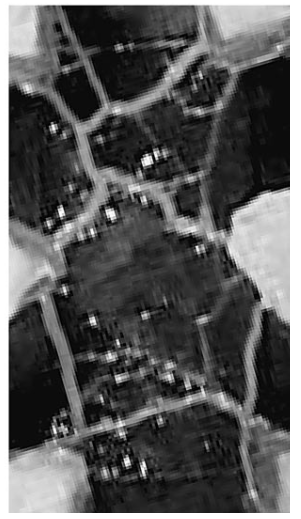
\includegraphics[height=0.3\textheight,keepaspectratio]{mst/mst_b.png}}
				\subfloat[Network formation experiment - Optimal MST][]{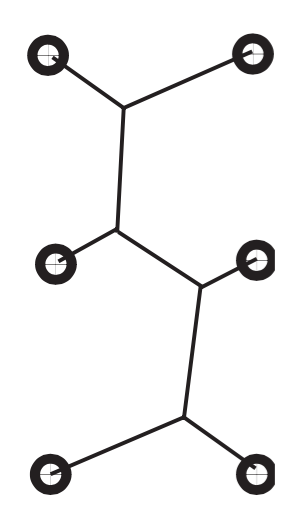
\includegraphics[height=0.3\textheight,keepaspectratio]{mst/mst_c.png}}
				\caption[Network of food sources by \P]{ (a) A network resembling the minimum Steiner tree connecting six food sources (\textbf{\texttt{FS}}) laid out in a regular pattern. (b) An example of a network with a SMT-like pattern in the upper half and a cycle of veins in lower half. (c) A sample minimum Steiner tree on six nodes. Reprinted from~\cite{nakagaki2004obtaining}.}
				\label{fig:steiner_tree_experiment}
			\end{figure}

			\FloatBarrier

		\subsubsection{Minimizing Risk Associated with Illumination}

			In 2007 the plasmodium of \P was challenged with a different variant of optimization problem involving the organisms strong tendency to avoid light. 

			In the experiment the plasmodium is allowed to spread evenly across a rectangular petri dish. Next, two food sources are introduced at two adjacent corners of the container and a fraction of the container is evenly illuminated with white light. When the whole container is illuminated \P forms a thick vein connecting the two food sources, approximating the shortest path between them. If only a fraction of the container is illuminated, \P still connects the two food sources forming a thick vein. However, now the organism is trying to minimize its exposure to light by striking a balance between short connection and a short path through the illuminated area. In fact, the behavior of \P in this experiment is strikingly similar to the behavior of refracting light as given by Snell's law. \Fref{fig:snell} illustrates the experiment.

			The illumination experiments yet again demonstrate the uncanny ability of \P to solve complex problems. Furthermore, it shows that the behavior of \P can be effectively steered using light. Together with the potential to use chemical attractants and repellents, rich possibilities of controlling the behavior of the slime mold are available.

			\begin{figure}[htp]
				\centering
				\subfloat[Illumination experiment - Initial state][]{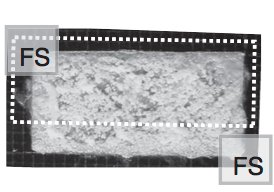
\includegraphics[width=0.45\linewidth,keepaspectratio]{snell/experiment_panel_a.png}\label{fig:snell:a}}
				\subfloat[Illumination experiment - Partial illumination][]{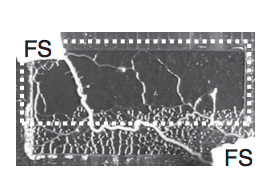
\includegraphics[width=0.45\linewidth,keepaspectratio]{snell/experiment_panel_d.png}\label{fig:snell:d}}
				\newline
				\subfloat[Illumination experiment - Full illumination control][]{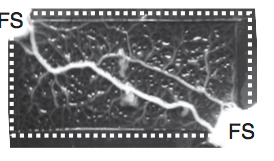
\includegraphics[width=0.45\linewidth,keepaspectratio]{snell/experiment_panel_b.png}\label{fig:snell:b}}
				\subfloat[Illumination experiment - Partial illumination][]{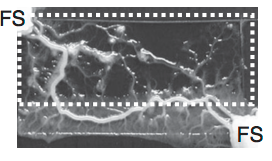
\includegraphics[width=0.45\linewidth,keepaspectratio]{snell/experiment_panel_e.png}\label{fig:snell:e}}
				\newline
				\subfloat[Illumination experiment - Full illumination control][]{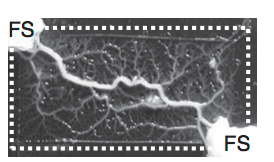
\includegraphics[width=0.45\linewidth,keepaspectratio]{snell/experiment_panel_c.png}\label{fig:snell:c}}
				\subfloat[Illumination experiment - Partial illumination][]{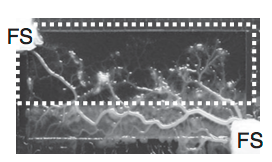
\includegraphics[width=0.45\linewidth,keepaspectratio]{snell/experiment_panel_f.png}\label{fig:snell:f}}

				\caption[Classic maze experiment with \P]{(a)  The  rectangular  sheetlike  morphology  of  the organism  immediately  before  the  introduction  of  two  food sources (\textbf{\texttt{FS}}). The region affected by illumination is indicated by a dashed rectangle. In (c) and (d) the entire region was illuminated. As a result an the shortest path between the two food sources is approximated by a thick vein. In (b), (d) and (f) partial illumination leads to a reduced path length through the illuminated area at the expense of an increase in total path length. Note the natural variation in the exhibited paths from experiment to experiment. Reprinted from~\cite{PhysRevLett.99.068104}.}
				\label{fig:snell}
			\end{figure}

			\FloatBarrier

	\subsection{Natural Computing Approaches}

		After a short survey of key experimental observations presented in the previous section, we move on to discuss common strategies to use the plasmodium of \P as a medium for natural computing. Here we present examples for the different paradigms discussed in the section natural computing. In the interest of brevity, we focus on the most successful approaches and refer the reader to the literature for details.

		% The first approach consists of modeling some aspect of \P with the goal of using this model for \textit{in silico} computation. The major challenge here is to look past the intricate bio-physical processes that are observed experimentally and find a suitable level of abstraction capable of capturing the computational abilities of \P
		% Once a reliable model has been established, its suitability to solve computational problems can be studied. Since most of the resulting computational algorithms are comparably complicated, they frequently resist theoretical analysis. However, in some cases the algorithms are well understood and convergence properties and runtime guarantees have been established.

		% The second approach seeks to realize computation with \P \textit{in vivo} by manipulating live plasmodium in such a way, that its reaction and evolution can be interpreted as computation.

		% In the following we present an incomplete selection of the most important approaches that have been successfully used to realize natural computing with \P.

		\subsubsection{Computing Inspired by P.~Polycephalum}

			The approach aims at modeling certain aspects of \P with the goal of using the resulting models for \textit{in silico} computation. The major challenge here is to look past the intricate bio-physical processes that are observed experimentally and find a suitable level of abstraction capable of reproducing the computational abilities of \P.
			
			Shortly after it was demonstrated that \P forms networks connecting more than two food sources, Nakagaki \etal went on to explain their own observations on a physiological level in~\cite{Tero2006115}. 

			They claim that the plasmodium of \P organizes itself through the formation of thick veins through which the protoplasm is driven as a result of periodic contractions of the veins themselves, \ie peristaltic pumping. Veins are formed when streaming of protoplasm persist in a given direction for a sufficiently long time~\cite{nakagaki2000interaction}. On a molecular scale Actomyosin fibers carried by the protoplasmic flow attach themselves to each other forming a mesh of fibers, eventually resulting in tubular structures. The fast flowing protoplasm causes shear stress, exerting a force which stretch-induces a regular orientation of the otherwise arbitrarily oriented fibers along the direction of flow. As a result, veins with a large flux manage to accumulate and orient even more Actomyosin fibers which over time lead to an increase in vein diameter. This in turn further reduces the resistance to flow, since under the assumption that the fluid flow in the veins of \P is a Poiseuille flow, the theory of hydrodynamics dictates that it be proportional to the forth power of the vein diameter and inverse proportional to the vein length. It follows that veins which are carrying little flow either are long and/or thin or happen to be dead-end veins. The latter are likely to degenerate over time as experimentally demonstrated in various experiments. At the same time, reinforcing thick and short veins increases the efficiency of fluid flow, which in turn enables effective circulation and transport of nutrients, nuclei and other factors.

			These considerations became the basis of a concise model presented in 2006, which captures the behavior of the slime mold as demonstrated in the maze experiment and lead to the first natural computing approaches based on \P~\cite{Tero2006115}. The model can be formulated on a graph $G = (V,E)$, where the node set $V$ denotes the junction points of veins and the edge set $E$ denotes the veins themselves. Each node $u \in V$ has a hydrodynamic pressure associated with it denoted by $p_u(t)$. Each edge $e = (u,v) \in E$ has a length $L_e$ as well as a time-dependent flow through the vein labeled $Q_e(t)$. Here it is assumed that the flow is a Poiseuille flow such that

			\begin{equation}
				Q_e(t) = \frac{\pi r_e(t)^4}{ 8 \eta} \frac{p_u(t)-p_v(t)}{L_e}\,,
				\label{eq:flow_initial}
			\end{equation}
			holds. Here $r_e(t)$ is the diameter of an edge and $\eta$ refers to the viscosity of the protoplasmic fluid. Let $D_e(t) = \pi r(t)^4/ 8 \eta$. Then we can simplify \Fref{eq:flow_initial} to read

			\begin{equation}
				Q_e(t) = \frac{D_e(t)}{L_e} (p_i(t) - p_j(t))\,.
				\label{eq:flow}
			\end{equation}

			Let us choose two distinct nodes $s, t \in V$ representing the source and sink nodes in the graph. Using this definition we obtain an equation for each edge $e \in E$:

			\begin{equation}
				\sum_{e = (u,v) } Q_e(t) =
				\begin{cases}
				\quad 1 & \ \text{for} \ u=s\,, \\
				\quad -1 & \ \text{for} \ u=t\,, \\
				\quad 0 & \ \text{otherwise}\,.
				\end{cases}
				\label{eq:conservation_of_flow}
			\end{equation}
			
			Note that the l.h.s is chosen such that flow is conserved everywhere except at the source and the sink where flow is entering respectively leaving the graph. Thus one unit of flow is introduced to the system. \Fref{eq:conservation_of_flow} can be solved to obtain the values of the $Q(t)_e$ and the $p_u(t)$ simultaneously.

			Finally the time-dependence of $D(t)_e$ is choose such, that the positive feedback between $D(t)_e$ and $Q_e(t)$ is as described above. For each $e \in E$ the dimensionless equation for $D(t)_e$ reads

			\begin{equation}
				\frac{d}{dt} D_e(t) = f( Q(t)_e ) - D_e(t)\,,
				\label{eq:evolution}
			\end{equation}
			which is called adaptation or \emph{evolution equation}. Here $f$ is a monotonically increasing continuous function such that $f(0) = 0$. \Fref{eq:evolution} is the key of the model which formalizes the experimental observations reported earlier. If at time $t$ the flux through an edge is such that $f(Q_e(t)) < D_e(t)$ then $D_e(t)$ decreases which further reduces the flux through $e$. In this scenario an edge $e$ is degenerating. Likewise $f(Q_e(t)) > D_e(t)$ leads to an increase in $D_e(t)$ which further increases the flux. In this case $e$ is reinforced. Only ,$f(Q_e(t)) = D_e(t)$ enables a stationary state which leaves $D_e(t)$ and $Q_e(t)$ constant. 

			The model thus evolves the thickness of veins in \P according to \Fref{eq:evolution} relying on the values of $p_u(t)$ and $Q_e(t)$ which are governed by \Fref{eq:conservation_of_flow}. For suitable choices of $f(Q_e)$ this system can be discretized and solved numerically~\cite{Tero2006115}. For the graph depicted in~\Fref{fig:maze:abstraction} a stationary state was found where the $D_e(t)$ of all edges that do not belong to the shortest path between $s=N_1$ and $t=N_2$ vanished. At the same time $D_e(t)$ of the edge on the shortest path approached a constant. That is, just like the slime mold, the model has selected the shortest path in the graph between $s$ and $t$. 

			After this initial demonstration of the viability of \P as a medium for natural computing, mathematicians and computer scientists started to analyze the model and its variants contributing a sequence of convergence proofs and complexity bounds. For suitable choices of $f(Q_e)$ convergence was proven for planar graphs at first~\cite{miyaji2007mathematical,miyaji2008physarum}, but shortly thereafter proofs were extended to general graphs for the original model and for variations thereof~\cite{bonifaci2012physarum,bonifaci2013physarum,ito2011convergence,becchetti2013physarum}. The fact that the theoretical properties of the so-called \emph{Physarum solver} are rather well understood is a rarity amongst natural computing algorithms.

			Due to its success and intuitive basic idea, the Physarum solver has received much interest in the scientific community. Subsequently it inspired several other algorithms with varying degree of similarity to the original problem. An incomplete selection is given in \Fref{tab:list_inspired}. 

			\begin{table}
				\centering
				\begin{tabular}{@{} l *2c @{}}
				\toprule
				 \multicolumn{1}{c}{Problem}    & Authors  & Year   \\ 
				\midrule
				 Transport network design & Tero \etal~\cite{tero2010rules} & 2010 \\
				 Linear programs & Johannson \etal~\cite{Johannson2012} & 2012  \\ 
				 Learning Bayesian network structure & Sch\"on \etal~\cite{schon2012structure} & 2012  \\ 
				\bottomrule
				\end{tabular}
				\caption[Computing inspired by \P]{Various problems and related solution strategies inspired by the original Physarum solver.}
				\label{tab:list_inspired}
			\end{table}

			\FloatBarrier

		\subsubsection{Synthesis of P.~Polycephalum Using Computation}

			This approach seeks to faithfully synthesize \P by means of simulation. To do so, it relies on a suitable model capable of mimicking the behavior of the organism. Contrary to the approach presented in the previous section, finding a model that solves a computational problem is not the main goal. However, it has been shown that in the case of \P accurate modeling of the organism produces a model with problem solving capabilities. 

			In 2010 Jones suggested to take a closer look towards the foraging behavior of \P, emphasizing its ability to move towards food based on sensing chemicals signaling its presence~\cite{jones2010characteristics}. In particular he puts forward the idea of modeling the plasmodium of \P as a virtual 2D material consisting of a large population of virtual agents. These agents reside on a 2D lattice whose nodes store the concentration of a hypothetical chemical representing the presence of food. Agents are equipped with sensors that allow them to orient themselves towards the locally strongest concentration $c$ of this chemical in the lattice. After reorientation the agent deposits a chemical concentration equal to $c$ at its current location and then takes a step forward. This behavior effectively couples neighboring agents with each other, since they read and react to the trails of chemicals that are being deposited by others. A similarity with the general idea of ant colony optimization is observed. Figure \Fref{fig:agent} depicts a schematic of an agent and its sensors.

			\begin{figure}
				\centering
				\subfloat[Oscillator experiment - Plasmodium][]{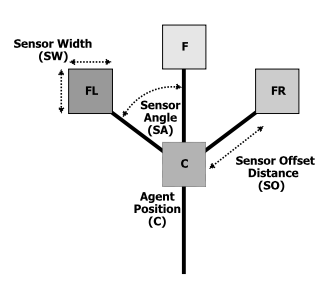
\includegraphics[width=0.45\linewidth,keepaspectratio]{agents/agent.png}}
				
				\caption[Multi-agent \P \ - Agent schematic]{Structure of a virtual agent showing central position and $3$ forward-facing offset sensors. Reprinted from~\cite{jones2010characteristics}.}
				\label{fig:agent}
			\end{figure}

			Given suitable parameters settings, the collective behavior of all agents leads to the spontaneous formation of transport networks. The emergent global patterns formed by the collective of agents resemble the actin-myosin mesh structures forming the veins of \P, while the individual trajectories of the agents can be interpreted as protoplasmic fluid flowing through the veins of the organism, see \Fref{fig:agent_structures}. \Fref{fig:agent_evolution} shows how an initially randomly distributed collection of agents evolves in time to eventually form a network. In particular, certain parameters of the model can be tuned such that the collective demonstrates minimization processes observed in~\cite{jones2011influences,jones2015applications,baumgarten2015network}. 

			\begin{figure}
				\centering
				\subfloat[Oscillator experiment - Plasmodium][]{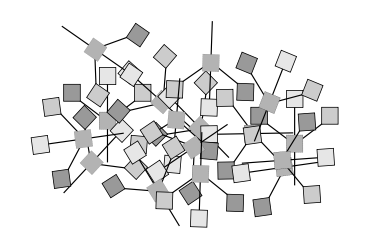
\includegraphics[width=\twoimageswide,keepaspectratio]{agents/agent_structure.png}}
				\subfloat[Oscillator experiment - Plasmodium][]{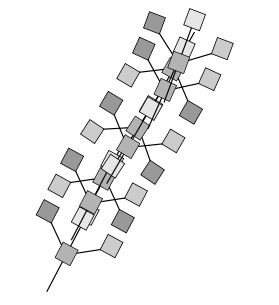
\includegraphics[width=\twoimageswide,keepaspectratio]{agents/agent_flow.png}}
				
				\caption[Multi-agent \P \ - Collective behavior of agents]{(a) A static collective of agents approximates plasmodium actin-myosin mesh. (b) A mobile stream of agents approximates protoplasmic flow within the plasmodium. Caption and figures reprinted from~\cite{jones2010characteristics}.}
				\label{fig:agent_structures}
			\end{figure}

			\begin{figure}
				\centering
				\subfloat[Oscillator experiment - Plasmodium][]{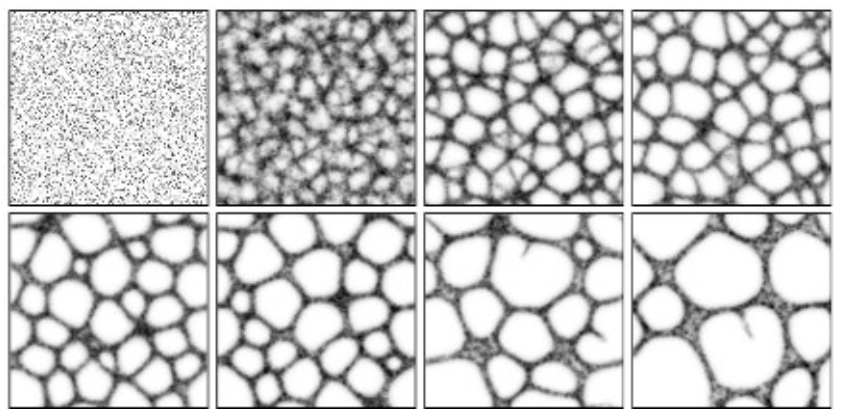
\includegraphics[width=\oneimagewide,keepaspectratio]{agents/evolution.png}}
				
				
				\caption[Multi-agent \P \ - Evolution of agents]{The coupling of agents with each other causes spontenous formation and evolution of transport networks. Reprinted from~\cite{jones2016multi}.}
				\label{fig:agent_evolution}
			\end{figure}

			In~\cite{jones2016multi} it is pointed out that pattern formation in itself does not yet constitute computation. Thus inspired by previous experimental results, it was suggested to add additional external stimuli to the lattice. These act as the input and the constraints necessary for a controlled computation. They can be attractants or repellents which are projected onto the lattice and create concentration gradients which agents may react to. The placement of additional stimuli acts as constraints to the natural minimization process realized by the virtual material. The constrained process may be interpreted as computation. It is halted once the material has reached a stable configuration which is then interpreted as the solution or the output of the computation.

			An example of this approach can be seen in \Fref{fig:agent_mst} where six attractants where projected onto the chemo-attractant lattice. They correspond to food sources representing the input to the virtual \P experiment. When the virtual material is introduced it undergoes morphological changes constrained by the input. After a certain number of iterations the configuration has stabilized, revealing a minimum Steiner tree.

			Further examples of problem solving by synthesizing \P \emph{in silico} are given in \Fref{tab:list_synthesize}.

			\begin{figure}
				\centering
				\subfloat[Oscillator experiment - MST][$t=0$]{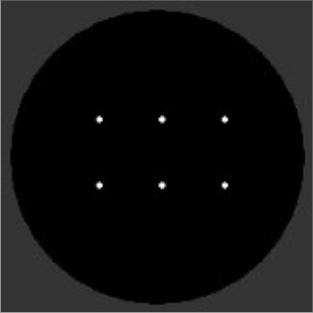
\includegraphics[width=0.3\linewidth,keepaspectratio]{agents/mst/1.png}}
				\subfloat[Oscillator experiment - MST][$t=40$]{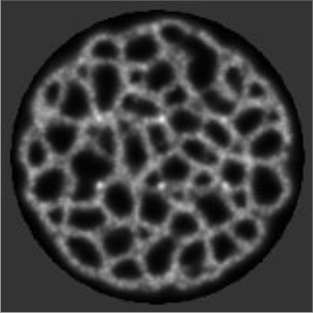
\includegraphics[width=0.3\linewidth,keepaspectratio]{agents/mst/2.png}}
				\subfloat[Oscillator experiment - MST][$t=350$]{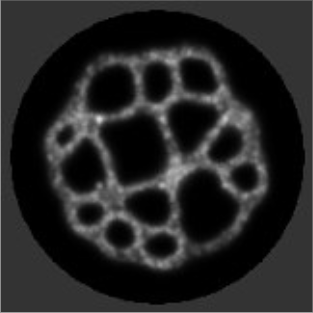
\includegraphics[width=0.3\linewidth,keepaspectratio]{agents/mst/3.png}}
				\newline
				\subfloat[Oscillator experiment - MST][$t=850$]{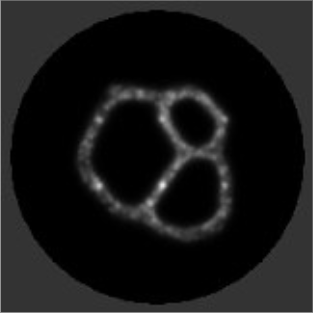
\includegraphics[width=0.3\linewidth,keepaspectratio]{agents/mst/4.png}}
				\subfloat[Oscillator experiment - MST][$t=1500$]{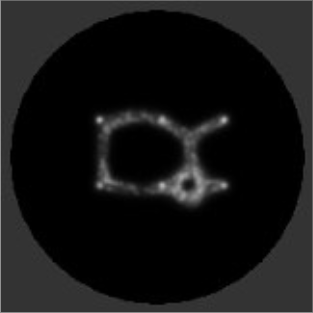
\includegraphics[width=0.3\linewidth,keepaspectratio]{agents/mst/5.png}}
				\subfloat[Oscillator experiment - MST][$t=5000$]{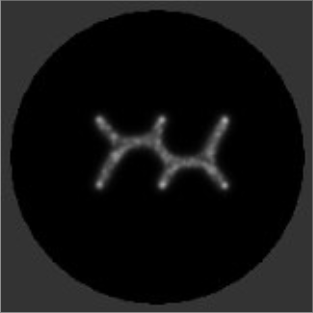
\includegraphics[width=0.3\linewidth,keepaspectratio]{agents/mst/6.png}}
				
				
				\caption[Multi-agent \P \ - Evolution of agents]{Material computation by constraining pattern formation. (a) A pattern of six nodes inside a circular arena is projected into the diffusive lattice as attractant stimuli. (b) Spontaneous formation of a transport network from random inoculation positions realized with 4000 particles. (c)-(e) The minimization of the network is constrained by the attraction to nodes. (f) The final stable configuration (output) is a Steiner minimum tree. Caption and figure adapted from~\cite{jones2016multi}.}
				\label{fig:agent_mst}
			\end{figure}

			\begin{table}
				\centering
				\begin{tabular}{@{} l *2c @{}}
				\toprule
				 \multicolumn{1}{c}{Problem}    & Authors  & Year   \\ 
				\midrule
				 Cellular atutomata & Gunji \etal~\cite{gunji2008minimal,gunji2011adaptive}  & 2008,2011 \\ 
				 Voronoi diagrams & Jones \etal~\cite{jones2015slime} & 2013 \\ 
				 Traveling salesman & Jones \etal~\cite{jones2014computation} & 2014 \\ 
				 Data smoothing and filtering & Jones \etal~\cite{jones2014material} & 2014 \\ 
				 Convex and concave hull & Jones \etal~\cite{jones2016multi} & 2016 \\ 
				
				


				\bottomrule
				\end{tabular}
				\caption[Computing by synthesis of \P]{Various problems and related solution strategies obtained via synthesis of \P.}
				\label{tab:list_synthesize}
			\end{table}

			\FloatBarrier

		\subsubsection{Computing with Live P.~Polycephalum}

			In order to realize computation with live \P, the plasmodium may be interpreted as a parallel amorphous biological computing system. Here input is encoded via the spatial configuration of food sources. The slime mold reacts to the presented stimuli in a dynamic process which is interpreted as computation. Finally, once the organism has settled in response to the input, the configuration of its vein network is interpreted as the output of the process. The initial experiments conducted by Nakagaki \etal can be considered the first deliberate realizations of natural computing with \P as a computing medium. Soon thereafter further possibilities to manipulate and steer the behavior of the plasmodium with chemical attractants, repellents and light where explored.  

			Two approaches, the perhaps most impressive, deserve to be mentioned separately. The first demonstrates an \textit{in vivo} solution to the problem of planning a transportation network connecting a set of cities. The second shows how a cleverly devised feedback-control system allows \P to act as an entirely different natural computing system, namely a neural network.

			Tero \etal cultivated \P in a Petri dish designed as a miniature replica of the greater Kanto region where oat flakes were placed at the locations of Tokyo and other major cities. Geographical constraints such as oceans, lakes and mountains were realized by means of a corresponding illumination mask. Since \P tends to avoid light, growth was restricted to the shaded areas. Under these conditions \P soon formed a network spanning all the food sources available in the shade. Surprisingly, the networks formed by \P were found to resemble the actual railway networks serving the Kanto region while balancing efficiency, fault tolerance and cost~\cite{tero2010rules}. 

			\begin{figure}
				\centering
				\subfloat[Tokyo railway experiment][]{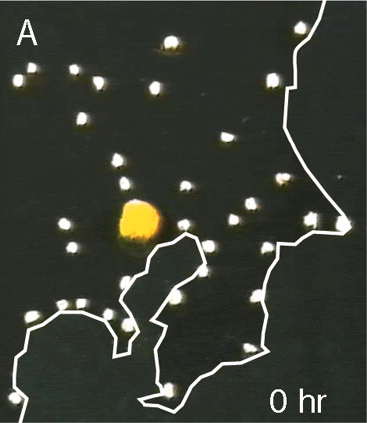
\includegraphics[width=0.3\linewidth,keepaspectratio]{jr/A.png}}
				\subfloat[Tokyo railway experiment][]{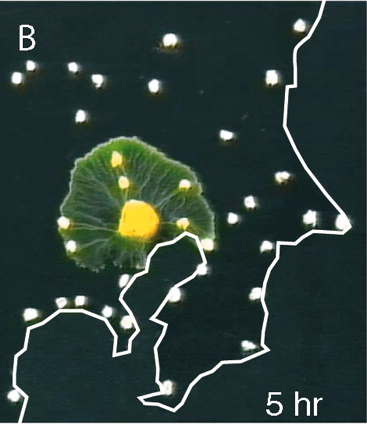
\includegraphics[width=0.3\linewidth,keepaspectratio]{jr/B.png}}
				\subfloat[Tokyo railway experiment][]{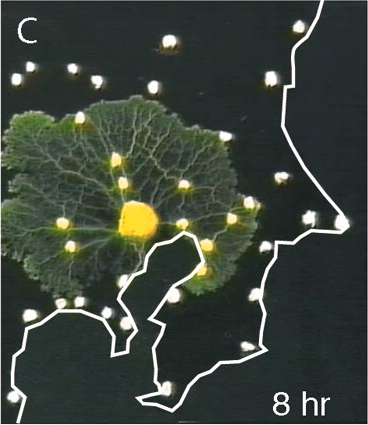
\includegraphics[width=0.3\linewidth,keepaspectratio]{jr/C.png}}
				\newline
				\subfloat[Tokyo railway experiment][]{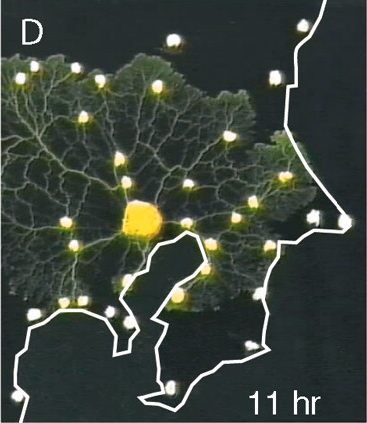
\includegraphics[width=0.3\linewidth,keepaspectratio]{jr/D.png}}
				\subfloat[Tokyo railway experiment][]{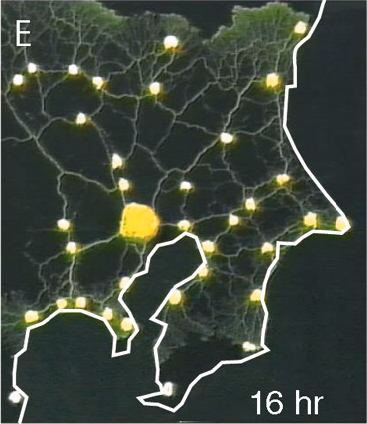
\includegraphics[width=0.3\linewidth,keepaspectratio]{jr/E.png}}
				\subfloat[Tokyo railway experiment][]{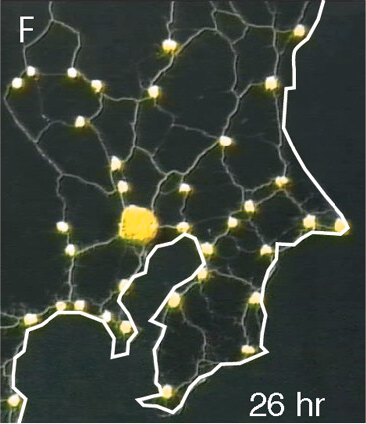
\includegraphics[width=0.3\linewidth,keepaspectratio]{jr/F.png}}
				
				
				\caption[Tokyo railway experiment]{Network formation in \Pp. (a) At $t = 0$, a small batch of plasmodium was placed at the location of Tokyo in an experimental arena bounded by the Pacific coastline (white border) and supplemented with additional food sources at each of the major cities in the region (white dots). The horizontal width of each panel is $17$ cm. (b) to (f): The plasmodium grew out from the initial food source with a contiguous margin and progressively colonized each of the food sources. Behind the growing margin, the spreading mycelium resolved into a network of tubes interconnecting the food sources. Caption and figure reprinted from~\cite{tero2010rules}.}
				\label{fig:tokyo}
			\end{figure}

			The experiment impressively demonstrated that \P can compute a feasible solution to the complex problem of designing a desirable real-life transport network, see \Fref{fig:tokyo}. Note that properly encoding the input by combining the location and quality of food sources as well as the illumination mask representing geographical constraints is critical. In addition to the \textit{in vivo} computation, Tero \etal also suggested a model based on the Physarum solver suitable for an \emph{in silico} replica of this experiment.

			\FloatBarrier

			While Tero \etal harvested the computing capabilities that follow from the natural foraging behavior and light-sensitivity of \P, Aono \etal suggest to trick \P into realizing a neural network~\cite{Aono:2007:ANC:1284621.1284651,Aono2009,Aono2007,Aono200883}. Their scheme is as follows: First, they design a star-shaped container where the ``legs'' of the container represent $8$ identical ``neurons'', see \Fref{fig:neurons_setup}. 

			\begin{figure}[!htbp]
			\centering
			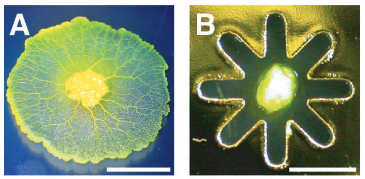
\includegraphics[width=\oneimagewide]{neurons/star_container.png}
			\caption[\P neurons - Setup]{L.h.s.: \P expanding unrestrictedly from an inoculation site. R.h.s.: \P placed in a star-shaped container. Scale bar equals \SI{2}{\milli\metre}. Reprinted from~\cite{Aono:2007:ANC:1284621.1284651}.}
			\label{fig:neurons_setup}
			\end{figure}

			When \P is placed inside the star it spreads equally across it. A neuron $x_i$ is considered active if more than a quarter of its area is occupied by the organism. Consequently, any neuron can be deactivated by illuminating its branch, which causes the plasmodium to retreat owing to its photo avoidance. The behavior of \P can be exploited to realize logical functions such as logical \textbf{\texttt{NOR}} by enforcing that a neuron $x_i$ be deactivated if any of its neighbors are active. 

			Thus, the exploring slime mold influences itself through the illumination pattern as it looks to occupy as large an area of possible. Under these conditions the plasmodium is lead towards certain configurations with a stable illumination pattern. When all neurons remain unchanged, the adopted configuration is interpreted as the output of the computation. \Fref{fig:neurons_states} shows various states the experimental setup can take.

			\begin{figure}[!htbp]
			\centering
			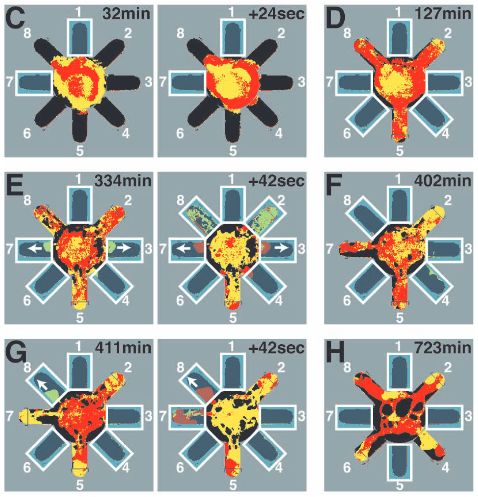
\includegraphics[width=\oneimagewide]{neurons/container_states.png}
			\caption[\P neurons - State transitions]{Time development of the \P neuron system. Illuminated branches of the container are indicated by white rectangles. The thickness oscillation phases are binarized as red and yellow for relaxing (thickness increasing) and contracting (decreasing) states, respectively. The l.h.s. row shows examples of transient states where the plasmodium is still exploring the container. The center row illustrates short term changes in thickness. The r.h.s. shows various stable configurations respecting different illumination patterns. Reprinted from~\cite{Aono:2007:ANC:1284621.1284651}. }
			\label{fig:neurons_states}
			\end{figure}

			Interestingly, the shape changes that the plasmodium undergoes in this setup may also be interpreted as state transitions in a McCulloch-Pitts neural network~\cite{Aono:2007:ANC:1284621.1284651}. Such networks have well studied computational capabilities and are known to be capable of approximating computational problems such as the traveling salesman problem. Exploiting the computational power of neural networks, Aono \etal demonstrated that \P can be used to realize an \textit{in vivo} computing system. Indeed, using an experimental setup with $N \times N$ branches it is possible to guide \P towards finding a solution for a TSP problem with $N=4$~\cite{Aono2009}. 

			This astonishing ability to guide and manipulate the behavior of \P is the key to various \textit{in vivo} computing systems devised so far, see \Fref{tab:list_invivo}.

			\begin{table}
				\centering
				\begin{tabular}{@{} l *2c @{}}
				\toprule
				 \multicolumn{1}{c}{Problem}    & Authors  & Year   \\ 
				\midrule

				Logic gates & Tsuda \etal~\cite{tsuda2004robust} & 2004 \\ 
				Robot control & Tsuda \etal~\cite{Tsuda2007215} & 2007 \\ 
				PhyChip: Growing computers from Slime Mould & Adamatzky \etal~\cite{adamatzky2012physarum} & 2012 \\ 
				
				\bottomrule
				\end{tabular}
				\caption[Computing with live \P]{Various applications of \P of as a living computing system.}
				\label{tab:list_invivo}
			\end{table}

			\FloatBarrier



